\section{Methodology}
\label{sec:method}

\subsection{Problem Formulation}
We formulate the Text-to-SQL task over a relational database $\mathcal{D} = (\mathcal{S}, \mathcal{V})$, where $\mathcal{S} = \{T_1, T_2, \ldots, T_M\}$ is the set of $M$ tables comprising the schema and $\mathcal{V}$ denotes the stored data values. Each table $T_j$ is characterised by its column set $\{c_{j,1}, \ldots, c_{j,|T_j|}\}$. Given a natural language question $Q$ and optional evidence hint $E$, the objective is to generate the optimal SQL query:
\begin{equation}
\label{eq:objective}
    \hat{y} = \arg\max_{y \in \mathcal{Y}} \; P_\theta\!\left(y \;\middle|\; Q, \mathcal{S}', \mathbf{C}_{\mathrm{meta}}, E\right)
\end{equation}
where $\mathcal{S}' \subseteq \mathcal{S}$ is the CHESS-pruned schema ($|\mathcal{S}'| = k \ll M$), $\mathbf{C}_{\mathrm{meta}}$ is the MCI metadata context, and $\theta$ denotes the LLM parameters.

\subsection{Architecture Overview}
As illustrated in Figure~\ref{fig:workflow}, the \texttt{MasterPipeline} orchestrates four sequential phases with a strict cost invariant:

\begin{quote}
    \textbf{Design Invariant}: A maximum of \textbf{3 LLM API calls} per question---Generation (call~\#1), Reflection (call~\#2), and conditional Correction (call~\#3). All schema pruning, metadata extraction, and semantic validation are executed locally at zero API cost.
\end{quote}

\begin{figure*}[t]
    \centering
    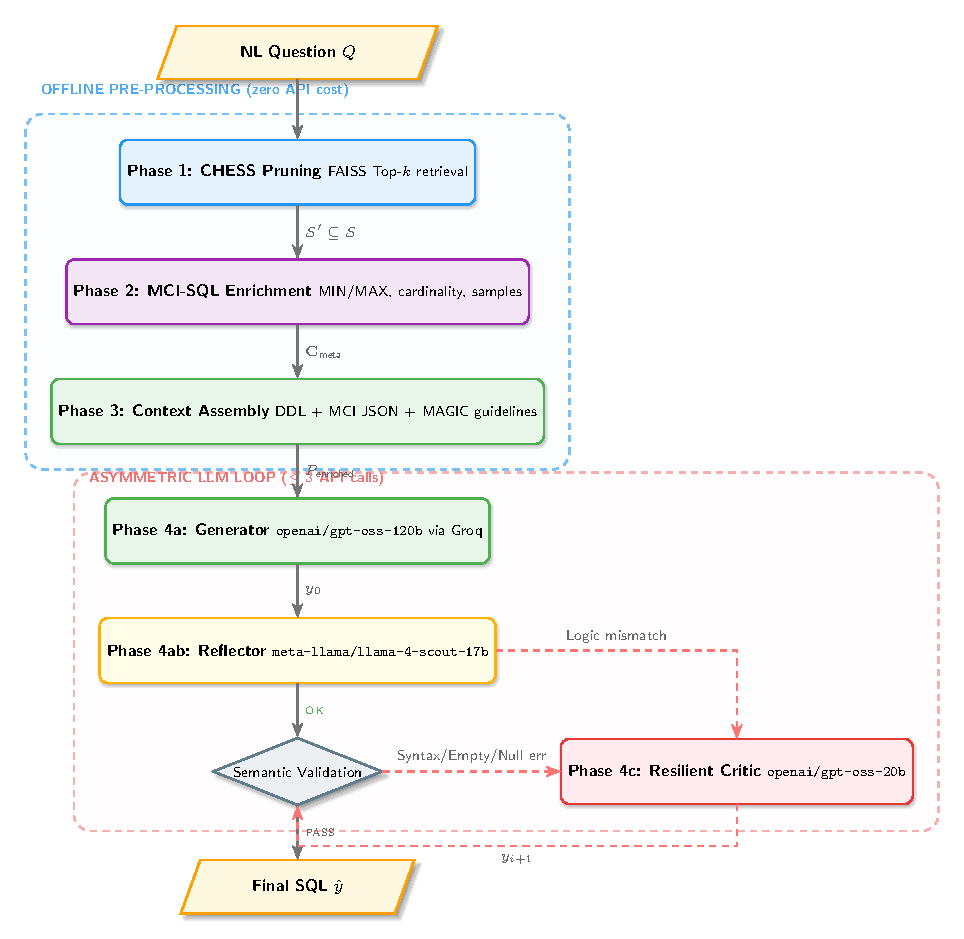
\includegraphics[width=0.88\textwidth]{tikz_artifacts/agentsql_workflow.pdf}
    \caption{The AgentSQL \texttt{MasterPipeline} architecture. Phases~1--3 (blue dashed box) run entirely offline against the local SQLite database. Phase~4 (red dashed box) implements the asymmetric LLM loop with at most 3 API calls: the Generator and Reflector use \texttt{llama-4-scout-17b} via Groq, while the Resilient Critic uses \texttt{gemini-2.5-flash} and is activated only on detected errors.}
    \label{fig:workflow}
\end{figure*}

\subsection{Phase~1: CHESS Semantic Pruning}
Given the question $Q$, we embed it using the BGE asymmetric query prefix and retrieve the Top-$k$ tables from a pre-built FAISS index \parencite{johnson2019faiss, xiao2024cpackpackedresourcesgeneral}:
\begin{equation}
\label{eq:chess}
    \mathcal{S}' = \operatorname{Top\text{-}k}_{T_j \in \mathcal{S}} \left\langle \mathbf{e}_Q, \; \mathbf{e}_{T_j} \right\rangle
\end{equation}
where $\mathbf{e}_Q = f_\theta(\texttt{``Represent this sentence: ''} \| Q)$ is the L2-normalised query embedding and $\mathbf{e}_{T_j}$ is the pre-computed table representation stored in the FAISS \texttt{IndexFlatIP}. The index is built \emph{once offline} by \texttt{build\_offline\_index.py}, encoding each table as a concatenation of its name, column names, and data-type declarations. This reduces the schema from $M$ tables to $k$ (default $k=3$), yielding a typical reduction ratio of 60--80\%.

\subsection{Phase~2: MCI-SQL Metadata Enrichment}
The \texttt{MetadataExtractor} profiles each column $c \in \mathcal{S}'$ locally via SQLite PRAGMA introspection and targeted queries:

\begin{itemize}
    \item \textbf{Numeric columns}: Extracts $\min(c)$ and $\max(c)$ for range validation.
    \item \textbf{Text columns}: Fetches $n_s = 3$ random non-null samples via \texttt{ORDER BY RANDOM() LIMIT 3} for literal value grounding.
    \item \textbf{Cardinality inference}: Computes $\frac{|\texttt{DISTINCT}(c)|}{|\texttt{COUNT}(*)|}$ to classify each column as \textsc{1:1 (PK-like)} or \textsc{1:N (FK/Categorical)}, guiding the LLM's join reasoning.
\end{itemize}
The result is a compact JSON string $\mathbf{C}_{\mathrm{meta}}$ with zero whitespace separators, minimising token consumption.

\subsection{Phase~3: Context Assembly}
Phases~1 and~2 are fused into a single enriched prompt $P_{\mathrm{enriched}}$:
\begin{equation}
\label{eq:prompt}
    P_{\mathrm{enriched}} = \texttt{DDL}(\mathcal{S}') \;\|\; \mathbf{C}_{\mathrm{meta}} \;\|\; \mathcal{G}_{\mathrm{MAGIC}} \;\|\; Q \;\|\; E
\end{equation}
where $\mathcal{G}_{\mathrm{MAGIC}}$ is an 8-rule MAGIC self-correction checklist \parencite{askari_magic_2024} covering common failure modes: \texttt{LIMIT/ORDER~BY} misuse, aggregation granularity, ratio casting, date format mismatches, join path validation, projection minimality, and extreme-value patterns.

\subsection{Phase~4: Asymmetric LLM Loop}
\label{subsec:asym_loop}

The pipeline enters the online LLM loop:

\subsubsection{Phase~4a: Generator}
A cost-efficient model $G$ (\texttt{llama-4-scout-17b} via Groq) produces the initial candidate:
\begin{equation}
    y_0 = G(P_{\mathrm{enriched}})
\end{equation}
The generator prompt forces a mandatory \texttt{<thought>} reasoning block declaring selected tables, join paths, and result grain before emitting the SQL.

\subsubsection{Phase~4ab: Reflector}
The same lightweight model $R$ performs a back-translation consistency check:
\begin{equation}
    R(Q, y_0) = \begin{cases}
        \texttt{<ok>}                     & \text{if SQL $\leftrightarrow$ NL consistent} \\
        \texttt{<error>}~\delta_{\mathrm{logic}} & \text{otherwise}
    \end{cases}
\end{equation}
where $\delta_{\mathrm{logic}}$ is a one-sentence description of the logical mismatch (e.g., ``\textit{Uses MIN instead of MAX for highest consumption}''). This catches silent logical errors that the database engine cannot detect.

\subsubsection{Phase~4b: Semantic State Evaluation}
If the Reflector approves, the SQL is executed locally by the \texttt{SemanticErrorChecker}, which classifies the outcome into one of four states:

\begin{table}[h]
    \centering
    \caption{Three-tier Semantic State Evaluation taxonomy.}
    \label{tab:semantic_states}
    \begin{tabular}{@{}lll@{}}
        \toprule
        \textbf{State} & \textbf{Trigger} & \textbf{Suggestion Strategy} \\
        \midrule
        \textsc{SyntaxError}  & \texttt{sqlite3.OperationalError} & Fix column/table name \\
        \textsc{EmptyResult}  & $|\mathrm{rows}| = 0$             & Use \texttt{LIKE} / \texttt{LOWER()} \\
        \textsc{NullResult}   & $\forall$ cells $= \texttt{NULL}$ & Fix JOIN ON clause \\
        \textsc{Valid}        & Non-empty, non-null rows          & Accept $\hat{y}$ \\
        \bottomrule
    \end{tabular}
\end{table}

\subsubsection{Phase~4c: Resilient Critic}
If \emph{any} error is detected (logical from Reflector or semantic from the checker), the Critic $C$ (\texttt{gemini-2.5-flash}) is invoked with the full error context:
\begin{equation}
    y_{i+1} = C\!\left(y_i, \; \delta_{\mathrm{error}}, \; \texttt{DDL}(\mathcal{S}'), \; \mathbf{C}_{\mathrm{meta}}, \; \mathcal{G}_{\mathrm{MAGIC}}\right)
\end{equation}
The corrected SQL is re-validated locally. The loop terminates when validation succeeds or the iteration budget $T_{\max} = 3$ is exhausted.

\subsection{System-Level Optimizations for High-Throughput}
Two engineering contributions underpin production reliability:
\begin{itemize}
    \item \textbf{Round-Robin \texttt{KeyRotator}}: Manages $N$ API keys per provider (e.g., $N=4$ Groq keys). On HTTP~429, the system rotates to the next key with \emph{zero sleep}, achieving sustained throughput during batch evaluations.
    \item \textbf{\texttt{ResilientGroqLLM} two-tier fallback}: If all $N$ keys are exhausted on the primary model (\texttt{gpt-oss-120b}), the factory transparently degrades to \texttt{llama-4-scout-17b} on the same key pool without pipeline interruption.
\end{itemize}
